\documentclass[a4paper]{article}
\usepackage[utf8]{inputenc}
\usepackage{fullpage}
\usepackage{amsmath,amssymb}
\usepackage[colorlinks]{hyperref} % use colored text in stead of ugly boxes
\usepackage[toc]{multitoc} % Nice two-column TOC

%~ \usepackage{enumerate} 
\usepackage{pgf}
\usepackage{tikz}
\usepackage{pictures/tikz-uml}

%~ \usepackage{listings}
%~ \lstset{language=java, tabsize=4, frame=single,basicstyle=\scriptsize}

\title{Programming Life - Requirements Analysis and Design }

\author{Group 5/E:\\
Felix Akkermans \\
Niels Doekemeijer \\
Thomas van Helden \\
Albert ten Napel \\
Jan Pieter Waagmeester}

\begin{document}
\maketitle

\vfill

\small{\tableofcontents}
\pagebreak
\section{Introduction} 		% (Niels)
The purpose of biotechnology is to use micro-organisms like moulds and bacteria for the production of chemical substances. These chemical substances are used as energy (biofuels), in products (bioplastics), in food and in medicine. Not only can these micro-organisms produce, they can also be used to break down chemical substances, for example in the purification of water.\footnote{Programming Life – Contextproject assignment (Dick de Ridder, Marcel Reinders)}

Using molecular biology, these micro-organisms can be altered to add, change or remove functionality. This is done by mutating the DNA of the organism. Synthetic biology is the science in which biology and engineering are combined to create new biological functionality\footnote{Programming Life – Contextproject kickoff (Dick de Ridder, Marcel Reinders)}. The engineering part is made easier by using biobricks\footnote{\url{http://biobricks.org/}}. These ``bricks" are simple genetic circuits which provide a basic functionality (for example the imitation of an OR or AND gate) and share a common interface. By combining these biobricks, a new biological systems can be engineered.

In its abstract form, this system can be visualized as a logical circuit, but in the organism the circuit corresponds with a group of molecules (proteins, genes, RNA) that react with each other. How (and if) they will react depends on many different elements, like the concentration and reaction speed of a protein. This reaction can be simulated using a (heavily) simplified model.\footnotemark[1]

In this report, we will describe the design of a visual modeling environment for synthetic biology, in which biotechnologists can design, simulate and validate a logical circuit built using biobricks. We will clarify our proposed system using a list of requirements (2.1), a few analysis models (2.4), a business object model (2.5), a few dynamic models (2.6) and a preliminary drawing of the interface (2.7). In chapter 3 we will give a planning of the following of the project.

\section{Proposed system}
\subsection{Overview} 		% (Niels)
In this document, we will provide an analysis and design proposal for a visual modeling environment for synthetic biology, in which biotechnologists can design, simulate and validate a logical circuit built using biobricks.

We have made up a list of requirements which answer the following questions.  What does the application have to do? What doesn't belong in the basic functionality? What kind of programming language will we use to develop this program and when is it due? First we will go into detail on functional requirements (2.2), so what does the program do? Secondly, we will discuss non-functional requirements (2.3). These answer questions like: What programming language will we use, but also how we will increase the usability of the application. Finally we will have a look at constraints (2.4).

Following the requirements we will specify a few use case models (2.5). These models describe specific scenarios of the program, what steps the user has to take to reach a goal and how the system should react to these steps. The main scenarios we will specify are loading/saving, modeling and simulating. Dynamic models such as sequence diagrams and activity diagrams will visualize the steps and interaction of the user and system in chapter 2.7.

Our business object model (2.5) will clarify the key concepts and their roles of our application. It will give a simplified overview of how proteins, biobricks and the System Biology Markup Language (SBML) relate to each other.

Last but not least, we will show a preliminary drawing of our interface (2.8) and explain why we have chosen for this interface and how it will work. Chapter 3 contains a planning for the rest of the project. This schedule is built up around the deadlines for the other documents and has a preliminary planning for the implementation fase.

\pagebreak
\subsection{Functional requirements}
The following are use cases the application must be able of completing in whatever way.

\begin{enumerate}
\item \textbf{Circuit abstraction} The application must be able to abstract a designed circuit into a BioBrick, and then treat this as a gate, so it can be used in building of subsequent circuits/BioBricks. 

\item \textbf{Protein specification} The user must be able to manually specify which protein is used to represent which signal in a circuit.

\item \textbf{Available proteins} The application must be able to present the user with an overview of available proteins to assign to signals. The available proteins must be predefined by a user.

\item \textbf{Export XML} The application must be able to export a built circuit as a BioBrick in XML (in the SBML schema).
\item \textbf{Import XML} The application must be able to import XML (in the SBML schema) into the application as a BioBrick.
\item \textbf{Interfering/invalid signals} The application must be able to notify the user that the current circuit design has protein(s) assigned to multiple signals, or still has signals which do not have a protein assigned.
\end{enumerate}

\subsection{Pseudo-requirements}
Non-functional requirements are requirements about how a the application behaves and operates (usability, accessibility, availability, performance). In this section we will also cover constraints on the source-code and development (programming language, documentation, tools/frameworks, compatibility, extensibility, maintainability, testability, deadlines).

\begin{enumerate}
\item \textbf{Documentation} For documentation we will use \LaTeX  to finalize the reports and will be written in English. GIT will be used for hosting and collaborating on documentation.
\item \textbf{Tools/frameworks} The use of other software development tools has not been decided upon yet.
\item \textbf{Testability} We want to be able to test every detail. We were discussion test drive development, but we have not fully decided upon that either. In any case, there should be a lot of tests, in the form of checks and sort of unit-tests, but also for user friendliness by real people.

\item \textbf{Usability} Because the program is not made for information technology students so we will spend some time increasing the usability. However, the target group consists of scientists, and to be more specific, mainly bio-informatics experts. Because of this we will not create step-by-step tutorials. Our aim is to make the application basic enough so that a regular scientist can work with the application.

\item \textbf{Extensibility} We want to create our application in such a way that BioBricks can be exported and re-used later as part of even greater BioBricks. As for the application, it is always best practice to make the application extendable, and so we shall aim for that.

\item \textbf{Maintainability} Maintainability is actually not one of our focuses. Because the application works on its own, and is only required to be developed until the end of this semester, this is not a major concern.

\item \textbf{Accessibility} Because our application frontend will be written for the web, we will host it somewhere and it should be accessible from anywhere, if there is internet. From the time of launch of our first version until the end of the project, there should always be a testable version hosted somewhere. It's also likely that we will use modern frameworks such as Bootstrap CSS to provide a high start-level of usability, although this has not been decided yet. The use of such well developed frameworks guarantees a high accessibility of the website.

\item \textbf{Deadline} The first version is up for evaluation on the fourth of May (04-05-212). The final version of the application is due on the fifteenth of June (15-06-2012).
\item \textbf{Biological plausibility} The application does \textit{not} have to give an biologically accurate or plausible simulation.

\item \textbf{Frontend} The GUI frontend of the application will be a website written in HTML+CSS+JavaScript. This means our application frontend will be compatible with all the big operating systems that support web browsers.\item \textbf{Backend} The backend will be written in Java Server Pages.
 
\end{enumerate}
\pagebreak
\subsection{Analysis models}
\subsubsection{Use case model, descriptions and scenarios}
\begin{figure}[h!]
	\caption{Use cases}
	\centering%simple use case, depending on tikz-uml
\begin{tikzpicture}
\begin{umlsystem}[x=4.5, y=4, fill=red!10]{Biobrick modeller/simulator}
        \umlusecase[y=-0.5, x=-1.5]{Start application}
        \umlusecase[y=-5.5, x=4]{Model Biobrick}
        \umlusecase[y=-8, x=4]{Simulate}
        \umlusecase[y=-3.5, x=4]{Export SBML}
        \umlusecase[y=-1.5, x=4]{Import SBML}
        
        \umlusecase[y=-7, x=10]{Specify protein}
        \umlusecase[y=-3, x=10]{View available proteins}
        
        \umlusecase[y=-9, x=0]{Quit application}
\end{umlsystem}

\umlactor{user}

\umlassoc{user}{usecase-1}
\umlassoc{user}{usecase-2}
\umlassoc{user}{usecase-3}
\umlassoc{user}{usecase-4}
\umlassoc{user}{usecase-5}
\umlassoc{user}{usecase-8}
\umlinclude{usecase-2}{usecase-6}
\umlinclude{usecase-2}{usecase-1}
\umlinclude{usecase-3}{usecase-1}
\umlinclude{usecase-4}{usecase-1}
\umlinclude{usecase-5}{usecase-1}
\umlextend{usecase-2}{usecase-3}
\umlextend{usecase-2}{usecase-7}

\end{tikzpicture}

\end{figure}
\subsection{Business Object model} % (Albert)
The objects of our model are the proteins, the biobricks, the circuits and the Systems Biology Markup Language.

The protein is the smallest building block of the model, with proteins and gates we can form Biobricks. These Biobricks can then be connected to each other to form a circuit. The Systems Biology Markup Language (SBML) can be used to represent and describe these circuits. So from the circuit the resulting SBML can be obtained and vice versa.
\begin{figure}[h!]
	\caption{Business Object model}
	\centering% documentation on tikz-uml:
% http://www.ensta-paristech.fr/~kielbasi/tikzuml/index.php?lang=en&id=doc#t-1.1
\begin{tikzpicture}

\umlclass{Protein}{
  concentration \\
  $K_m$ \\
  $n$ \\
}{}
\umlclass[y=-6]{BioBrick}{
  proteins \\
  gates \\
}{}
\umlclass[x=6,y=-6]{Circuit}{bricks[]}{}

\umlclass[x=6,y=0]{SBML}{circuit}{}



\umlassoc[mult1=*, mult2=*]{Protein}{BioBrick}
\umlassoc[mult1=*, mult2=*]{Circuit}{BioBrick}
\umlinherit[geometry=-|, arg1=represents,align1=right]{SBML}{Circuit}
\end{tikzpicture}


\end{figure}

\subsection{Dynamic models}

\pagebreak
\subsection{Interface} % (Jan Pieter)
To model a network of circuit from the basic gates provided, a simple GUI is proposed in figure \ref{fig-gui}. Three different actions can be performed in the main working area: adding wires, AND- and NOT-gates. For each wire/signal a protein can be selected.

The simulation can be run, and the result will be displayed in a simple graph.
\begin{figure}[h!]
	\label{fig-gui}	
	\caption{Quick mockup of the Graphical user interface}
	
		\centering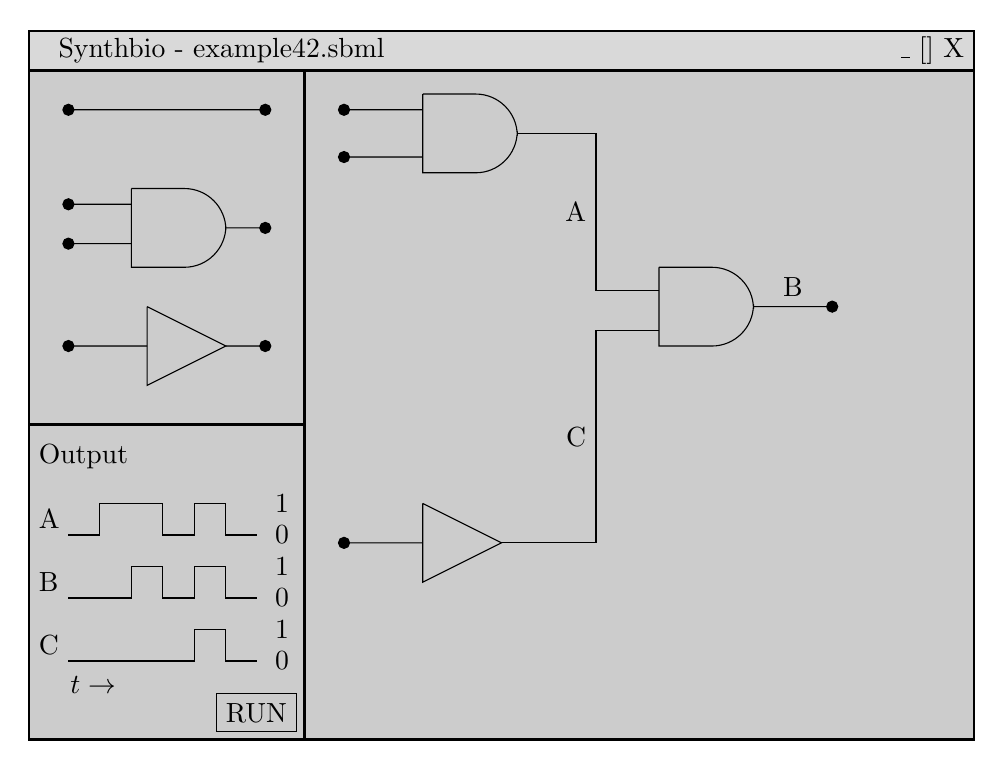
\begin{tikzpicture}

%main window
\draw[fill=black!20,line width=1] (-6,4) rectangle (6, -5);

% window title bar
\draw[fill=black!15,line width=1] (-6,4) rectangle (6, 3.5);
\node [anchor=west] at (-5.75, 3.75) {Synthbio - example42.sbml};
\node [anchor=east] at (6, 3.75) {\_ [] X};

% sidebar
\draw[fill=black!20,line width=1] (-6, 3.5) rectangle (-2.5, -5);
\draw[line width=1] (-6, -1) -- (-2.5, -1);

% wire
\draw (-5.5, 3) [fill]circle (2pt) -- ++( 2.5, 0) circle (2pt);

%and
\draw (-4.7, 2) [rounded corners=15pt] --  ++(1.2, 0)  -- ++(0, -1) [sharp corners] -- ++(-1.2, 0) -- ++(0, 1);
\filldraw (-5.5, 1.8) circle (2pt) -- (-4.7, 1.8);
\filldraw (-5.5, 1.3) circle (2pt) -- (-4.7, 1.3);
\filldraw (-3.5, 1.5) -- (-3, 1.5) circle (2pt);

%not
\draw (-4.5, 0.5) --  ++(1, -0.5) -- ++(-1, -.5) -- ++(0, 1);
\draw (-5.5, 0) [fill] circle (2pt) -- ++(1,0);
\draw (-3.5, 0) -- ++(.5, 0) [fill] circle (2pt);

%output
\node [anchor=west] at ( -6, -1.4) {Output};
\node [anchor=west] at(-5.6, -4.3) {$t \to$};

%signal A
\node [anchor=west] at ( -6, -2.2) {A};
\node [anchor=west] at ( -3, -2) {1};
\node [anchor=west] at ( -3, -2.4) {0};
\draw (-5.5, -2.4) -- ++(.4, 0) -- ++(0, .4) -- ++ (0.8, 0) -- ++(0, -.4) -- ++(.4, 0) -- ++(0, .4) -- ++(.4, 0) -- ++(0, -.4) -- ++(.4, 0);

%signal B
\node [anchor=west] at ( -6, -3) {B};
\node [anchor=west] at ( -3, -2.8) {1};
\node [anchor=west] at ( -3, -3.2) {0};
\draw (-5.5, -3.2) -- ++(.8, 0) -- ++(0, .4) -- ++ (0.4, 0) -- ++(0, -.4) -- ++(.4, 0) -- ++(0, .4) -- ++(.4, 0) -- ++(0, -.4) -- ++(.4, 0);

%signal C
\node [anchor=west] at ( -6, -3.8) {C};
\node [anchor=west] at ( -3, -3.6) {1};
\node [anchor=west] at ( -3, -4) {0};
\draw (-5.5, -4) -- ++(1.6, 0) -- ++(0, .4) -- ++ (0.4, 0) -- ++(0, -.4) --  ++(.4, 0);

%run button
\node [draw, anchor=south east] at (-2.6, -4.9) {RUN};

% Working area

%and gate
\draw (-2, 3) [fill]circle (2pt) -- ++(1, 0);
\draw (-2, 2.4) [fill]circle (2pt) -- ++(1, 0);
\draw (-1, 3.2) [rounded corners=15pt] --  ++(1.2, 0)  -- ++(0, -1) [sharp corners] -- ++(-1.2, 0) -- ++(0, 1);

%signal B
\draw (0.2, 2.7) -- ++ (1, 0) -- node[left] {A} ++(0, -2) -- ++(.8, 0);

%another gate
\draw (2, 1) [rounded corners=15pt] --  ++(1.2, 0)  -- ++(0, -1) [sharp corners] -- ++(-1.2, 0) -- ++(0, 1);

\draw (3.2, .5) -- node[above] {B} ++(1, 0) [fill] circle (2pt);

%not gate
\draw (-2, -2.5) [fill]circle (2pt) --  ++(1, 0);
\draw (-1, -2) --  ++(1, -0.5) -- ++(-1, -.5) -- ++(0, 1);

% signal C
\draw (0, -2.5) -- ++(1.2, 0) -- node[left] {C} ++(0, 2.7) -- ++ (.8, 0);

\end{tikzpicture}

	
\end{figure}

\pagebreak
\section{Planning}  % (Felix)

\pagebreak
\section{Glossary} % (Jan Pieter)
\begin{description}
	\item[BioBrick] Isolated and documented cell function to be reused in future projects. For example, the production of a light emitting protein when some other protein is available.
	\item[Circuit] What we think of as a circuit is actually just a cell wherein all signals and gates are proteins and parts of the DNA, mixed together without any separation.
	\item[DNA] \text{Deoxyribonucleic acid} is a very long molecule containing the information needed to support the life in allmost all creatures.
	\item[Protein] a complex molecule produces by certain processes in the cell. In turn it can activate other processes, or perform functions such as emission of light or change color.
	\item[RNA] Working copy of the information in the DNA. This copy is then used to synthesize proteins.
	\item[SBML] \textit{Systems Biology Markup Language} is a XML-based format for storage of various computermodels of biological processes.
	\item[Simulation] Execution of a set of differential equations in order to predict the output of the modelled circuit
	\item[Transcription] Process of making the mRNA-copy of the DNA master.
\end{description}
\end{document}